\documentclass[../index.tex]{subfiles}
\newglossaryentry{bintree}
{
    name=Бинарное дерево,
    description={Иерархическая структура данных, в которой каждый узел имеет не более двух потомков (детей). Как правило, первый называется родительским узлом, а дети называются левым и правым наследниками. Двоичное дерево не является упорядоченным ориентированным деревом}
}

\newglossaryentry{dyntree}
{
    name=Динамическое дерево,
    description={Иерархическая структура данных, в которой каждый узел имеет от 0 и более потомков (детей). Особенностью структуру является то что она не статическая и может произвольно изменяться(модифицироваться) внутренними узлами самой структуры}
}

\newglossaryentry{domelement}
{
	name=Элемент динамической формы,
	description={.}
}

\begin{document}

\section{Синтаксис}

Инструкции динамического языка представляют собой комбинации из конструкций всего двух типов: вызовов функций и литералов.

Основной конструкцией языка является \textit{функция}. Она состоит из имени и параметров. 
Сразу после имени функции следует символ '\verb|(|', за которым могут следовать один или 
несколько параметров, после этого вся конструкция завершается '\verb|)|', 
Некоторые функции вовсе не принимают параметры, см. листинг \ref{lst:lecsic} (1). 
Также поддерживается несколько параметров которые можно разделять символом '\verb|,|'
пример \ref{lst:lecsic} (2, 3), но не все среды выполнения (см. \autoref{environments}) 
поддерживают символ переноса строки, используя вместо него последовательность \verb|\r\n|.
Параметры функции можно переносить на следующую строку и добавлять пробелы для 
лучшей читаемости программы, \ref{lst:lecsic} (3)

Скобки после имени функции являются обязательными даже если у функции нет параметров.
Каждый параметр функции необходимо обернуть в '\verb|[|' '\verb|]|'.
Параметром функции может быть литеральное значение или вызов другой функции, вне зависимости от этого 
параметр необходимо обернуть в '\verb|[|' '\verb|]|'.

Литералы представляют собой константы, включаемые непосредственно в текст программы. 
Литералы не могут быть изменены в тексте программы.

Есть зарезервированный литерал $this$ который принимает значение id элемента на котором выполняется, 
подробнее в \autoref{sec:functions}.

\begin{figure}\label{lst:lecsic}
\begin{verbatim}
(1) func()

(2) func([arg0], [arg1], [argN])

(3) func(
        [arg0], [arg1]
        ,[arg2]
    )
\end{verbatim}        
\end{figure}

\section{Типы данных}\label{sec:types}

Динамический язык это зыком с динамической типизацией \footnotemark, определение типа происходит 
непосредственно перед передачей аргумента в функцию. 

\footnotetext {
динамическая типизация -- приём, широко используемый в языках программирования и языках спецификации, 
при котором переменная связывается с типом в момент присваивания значения, а не в момент объявления переменной.
}

Правила, по которым происходит приведение типа, следующие:

значение считается \textbf{числом}, если его строковое представление содержит только цифры и знак разделителя <<\verb|,|>> или <<\verb|.|>>.

значение считается  \textbf{логическим}, если строковое представление представляет собой последовательности \verb|true| или
 \verb|false|, вне зависимости от регистра символов.

В остальных случаях значением считается строкой символов.

%TODO *** Добавить примеры ***

\paragraph{Переменные}
Динамический язык не поддерживает определение и присвоение переменных. Однако функции позволяют изменять элементы 
динамической формы и значения в этих элементах можно считать своего рода переменными.

\section{Структуры данных}
Функции помимо литеральных значений могут принимать и возвращать определенные структуры данных Map и 3DMap.
Это необходимо для реализации вызова некоторых функций автоисполнятора (см. \ref{autoexec})

\textbf{Map} это структура данных \textbf{ключ} - \textbf{значение}. 
Обычно используется для хранения выбранного пункта в элементах типа \textbf{select} 
и \textbf{suggest} (см. \ref{suggest})
как правило ключ является идентификатором пункта, значение -- отображаемым пользователю текстом. Но для элементов
\textbf{suggest} применяются немного другие правила (см. далее).

\textbf{3DMap} -- структура данных для обмена дин формой между автоисполнятором и клиентской системой. 
Напрямую данную структуру использовать нельзя: она передается и принимается автоматически при вызове функций
название которых начинается с \verb|__| (два нижних подчеркивания). При вызове таких функций клиентский код, помимо передачи 
параметров функции, также передает информацию обо всех атрибутах дин. формы, а при ответе ожидает структуру, которая описывает
изменение атрибутов и значений существующих элементов, а также информацию об элементах которые необходимо добавить.
Примеры данных структур можно посмотреть в приложении \ref{apx:3dmap}

\label{sec:functions}
\section{Функции}

Функции позволяют выполнять действия на элементами формы, а также 
возвращать данные из контекста пользователя, шаблона или из другого элемента. 
Функции бывают нескольких типов: функции стандартной библиотеки, специальные, и асинхронные.

Как было отмечено ранее, функции могут принимать параметры и возвращать значения. 
Также у функции есть контекст выполнения: $this$ -- это литерал который в момент выполнения принимает значение id 
элемента, на котором выполняется данная команда.

\paragraph{Возвращаемые значения}

Все функции стандартной библиотеки динамического языка возвращают значение. Например,

\verb|getValue([foo])| -- вернет значение элемента, определяемого по идентификатору <<foo>> формы.

Функции, созданные для выполнения побочных эффектов, возвращают значение, как правило -- <<id>> элемента формы, над которым производится операция:

\verb|setValue([foo], [bar])| -- вернет <<bar>>

Даже функции, для которых в стандартной библиотеке возвращаемое значение не определено -- вернут пустой литерал: \verb|[]|


\subsection{Специальные функции}
Специальные функции предназначены для позволяют изменить путь выполнения программы с помощью ~if~, 
вызвать программу в контексте другого элемента -- ~call~.
Данные функции встроены в парсер и позволяют обойти ограничение простого вызова функций с параметрами.

Описание специальных функций:

\label{p:if}
\paragraph{if}
$if([conditon], [then], [else])$ -- позволяет выполнить динамический язык в зависимости от $condition$
$then$ $else$ не обязательные параметры

\label{p:run}
\paragraph{run}
$run([cmd0], \dotsc, [cmdN])$ -- вызывает аргументы функции и просто возвращает $true$. данная функция 
удобна когда нужно выполнить несколько команд ~параллельно~, и позволяет сократить вложенность команд.

\label{p:call}
\paragraph{call}
$call([command], [id])$ -- позволяет выполнить команду $command$ в контексте элементе с $id$, 
в данном случае $this$ внутри команды будет равен $id$. Если результат выполнения команды внутри CALL 
является динамической функцией создается дерево(см. \autoref{sec:execrules}) 
если результат не является динамической функцией - исходная команда внутри CALL. 
Выполняется над другим элементом динамической формы указанным во втором параметре функции CALL 

\label{p:string}
\paragraph{string}
$string(command)$ -- экранирует любой текст в рамках `(` `)`

\section{Порядок выполнения}\label{sec:execrules} 

В основе алгоритма определения порядка выполнения команд динамического языка лежит простая концепция -- выполнение функций должно происходить по слоям из самого глубокого вложенной функции к корневому элементу, при этом функция не может быть выполнена, пока не выполнены все ее дочерние элементы.

Итак поэтапно разберем последовательность действий происходящих при парсинге команд:
\begin{enumerate}
    \item Исходный строковый вид команды передается на вход анализатору, который содержит в себе регулярные выражения для парсинга
    \item Происходит валидация кода(в первых версиях реализации валидации не было), в случае ошибки валидации -- ошибки в количестве параметров функции, скобочках или невозможных символах - команда не будет выполнена и в лог действий будет выведена ошибка валидации
    \item Если команда успешно провалидирована, начнется построение динамического дерева(\gls{dyntree}). Важно отметить, что в ходе выполнения команды, дерево может менять свою структуру(\hyperref[sec:fif]{команда if}), а иногда даже создавать копии самого себя (\hyperref[sec:fcall]{CALL}). 
    \item Для построения динамического дерева используется стандартный левосторонний обход -- каждая следующая функция последовательно добавляется и спускается вглубь к следующему дочернему узлу, обойдя все элементы у первого дочернего узла, переходит ко второму, третьему и т.д.
    \item ПРИМЕЧАНИЕ. Особенными для разбора считаются функция IF, CALL и STRING в частности CALL и STRING останавливают дальнейший парсинг дочерних узлов функции и выставляют в результат строковое представление аргументов функции. Условная функция(оператор) IF -- разбирает изначально только первый дочерний узел, оставшиеся два так же сохраняет в строковых представлениях
    \item После разбора команды в динамическое дерево можно запускать ее на исполнение 
    \item В изначальной реализации динамического языка - динамическое дерево полностью преобразовывалось в очередь и выполняло все команды последовательно по кругу пока все функции не будут выполнены. В более современной реализации очередь содержит только активные элементы выполняющиеся непосредственно в текущей итерации и последовательно добавляет родительские узлы непосредственно в тот момент, когда имеется возможность их выполнить. Напомним, что родительский узел может быть выполнен только в случае когда все его дочерние команды вернули результат
    \item Выполнение начинается с самого глубокого уровня, если представить исходное динамическое дерево, то визуально его необходимо перевернуть и по слоям начать выполнять узлы дерева от листьев к корню, каждый следующий слой ожидает выполнения дочерних узлов предыдущего, в случае если функция является асинхронной, она не блокирует выполнение остальных команд на уровне
    \item ОСОБЕННОСТИ. Функции CALL и IF являются функциями модифицирующими динамическое дерево. Так функция CALL создает локальную копию поддерева их своих аргументов при этому есть два варианта(\hyperref[sec:fcall]{CALL})
    \item Функция IF на основе результата первого дочернего узла добавляет в исходное динамическое дерево либо второй, либо третий аргумент функции(третий может отсутствовать), происходит парсинг необходимой команды и динамическое дерево расширяется узлами дочерней функции внутри IF, параллельно выполняющейся в очереди начиная с уровня на котором размещен узел с IF(\hyperref[sec:fif]{подробнее про IF})
    \item В случае возникновения ошибок, возможны ситуации, которые прерывают дальнейшее выполнение команды.
    \item Результат корневого узла дерева обычно не используется и ничего не возвращает, за исключением  использование команды CALL.
\end{enumerate}
Для примера рассмотрим варианты динамических команд и представления в виде уровней и выполнения:

Рассмотрим команду 
\begin{verbatim}
    setValue(
        [10],
        [setEnable([true],
            [setVisible([true],[this])]
        )]
    )
\end{verbatim}

\begin{figure}[h]
	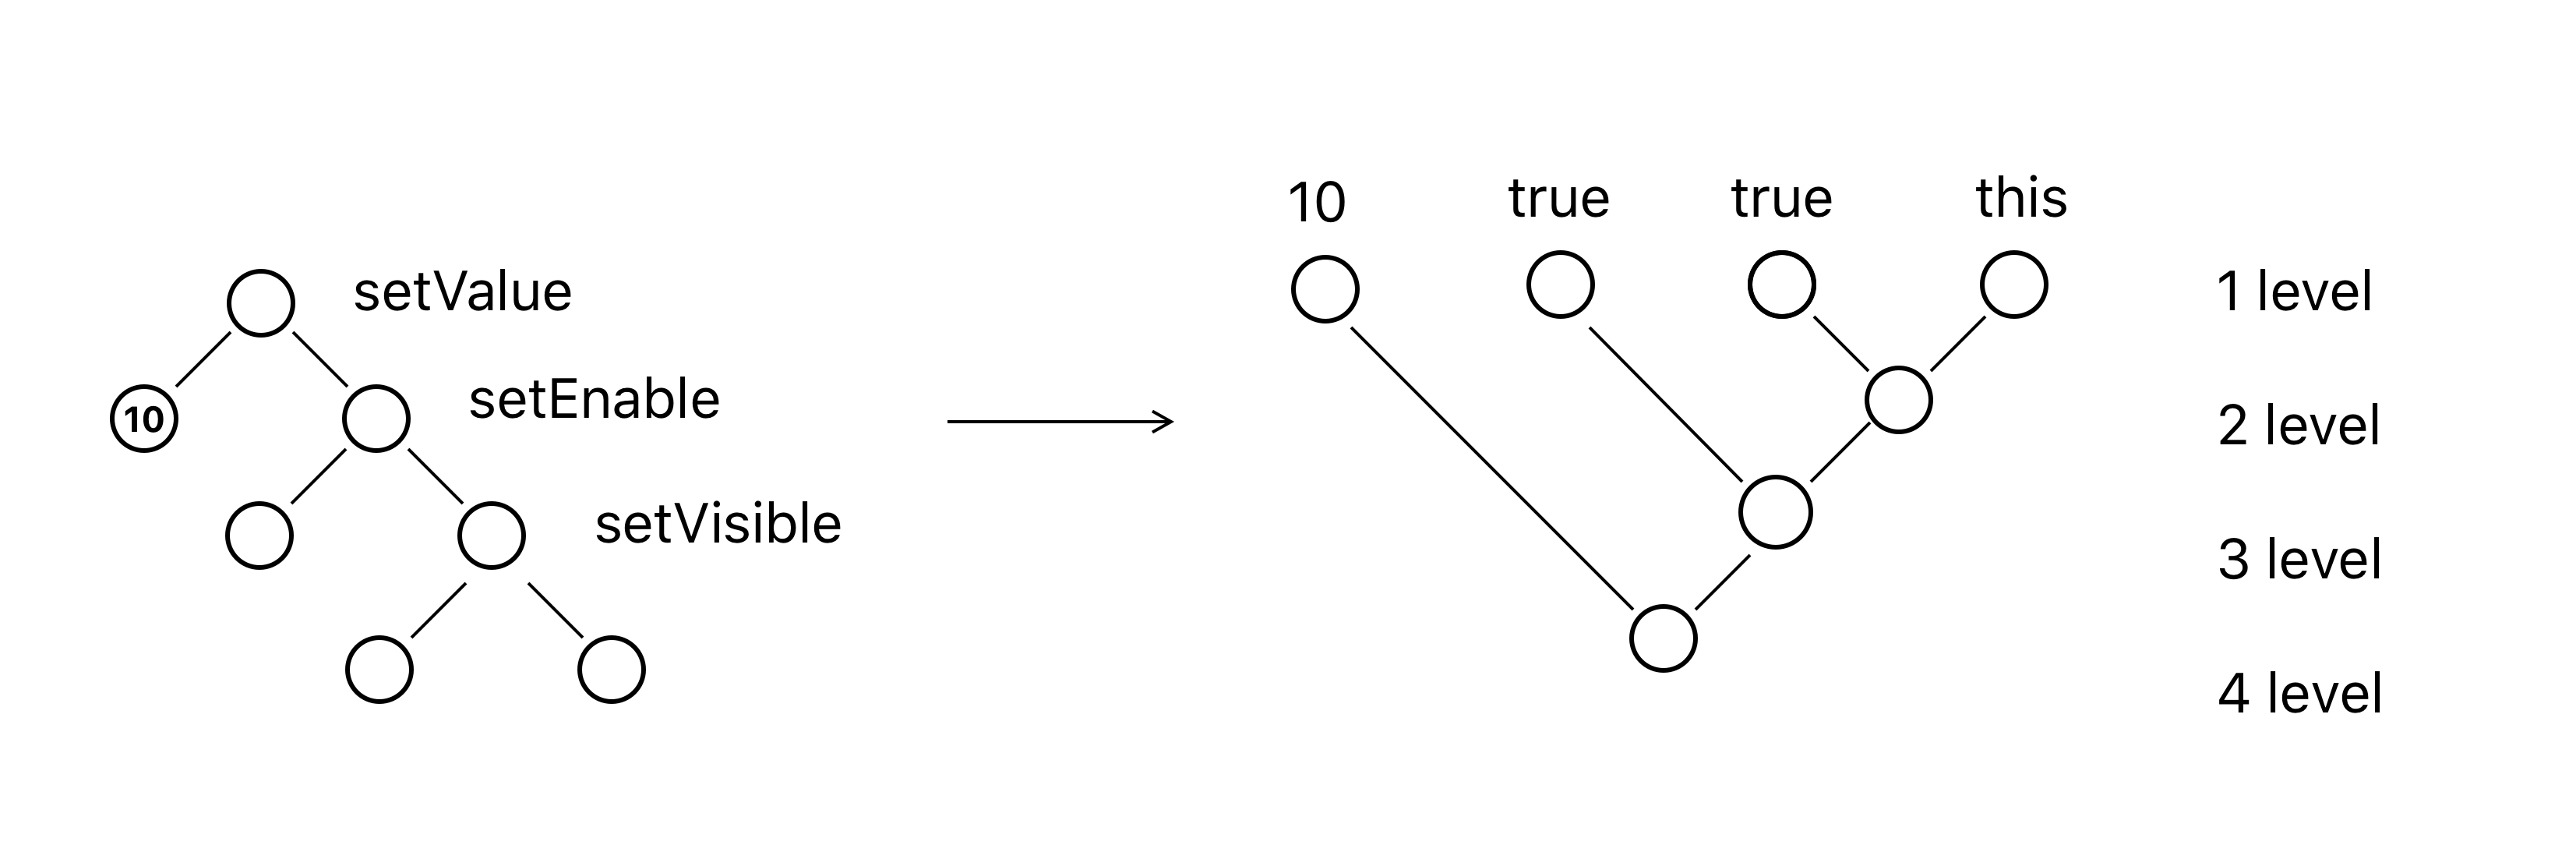
\includegraphics[width=1.0\textwidth]{simpleTree}
	\centering
\end{figure}
На изображении выше можно четко увидеть уровни по которым происходит выполнение команд, а теперь перейдем к более сложному варианту с использование функции $if$.

Для примера рассмотри абстрактную команду:
\begin{verbatim}
run(
    [if(
        [isin(
            [getValue([this])],
            [20],
            [10]
        )],
        [run(
            [setVisible([true],[this])],
            [setEnable([true],[this])],
        )],
        [setVisible(
            [false],
            [this]
        )]
    )],
    [setEnable(
        [true],
        [this]
    )]
)
\end{verbatim}
У функции $if$ три параметра, предположим, что результат первого выражения в $if$ истина, то порядок выполнения будет представлен следующим графиком:
\begin{figure}[h]
	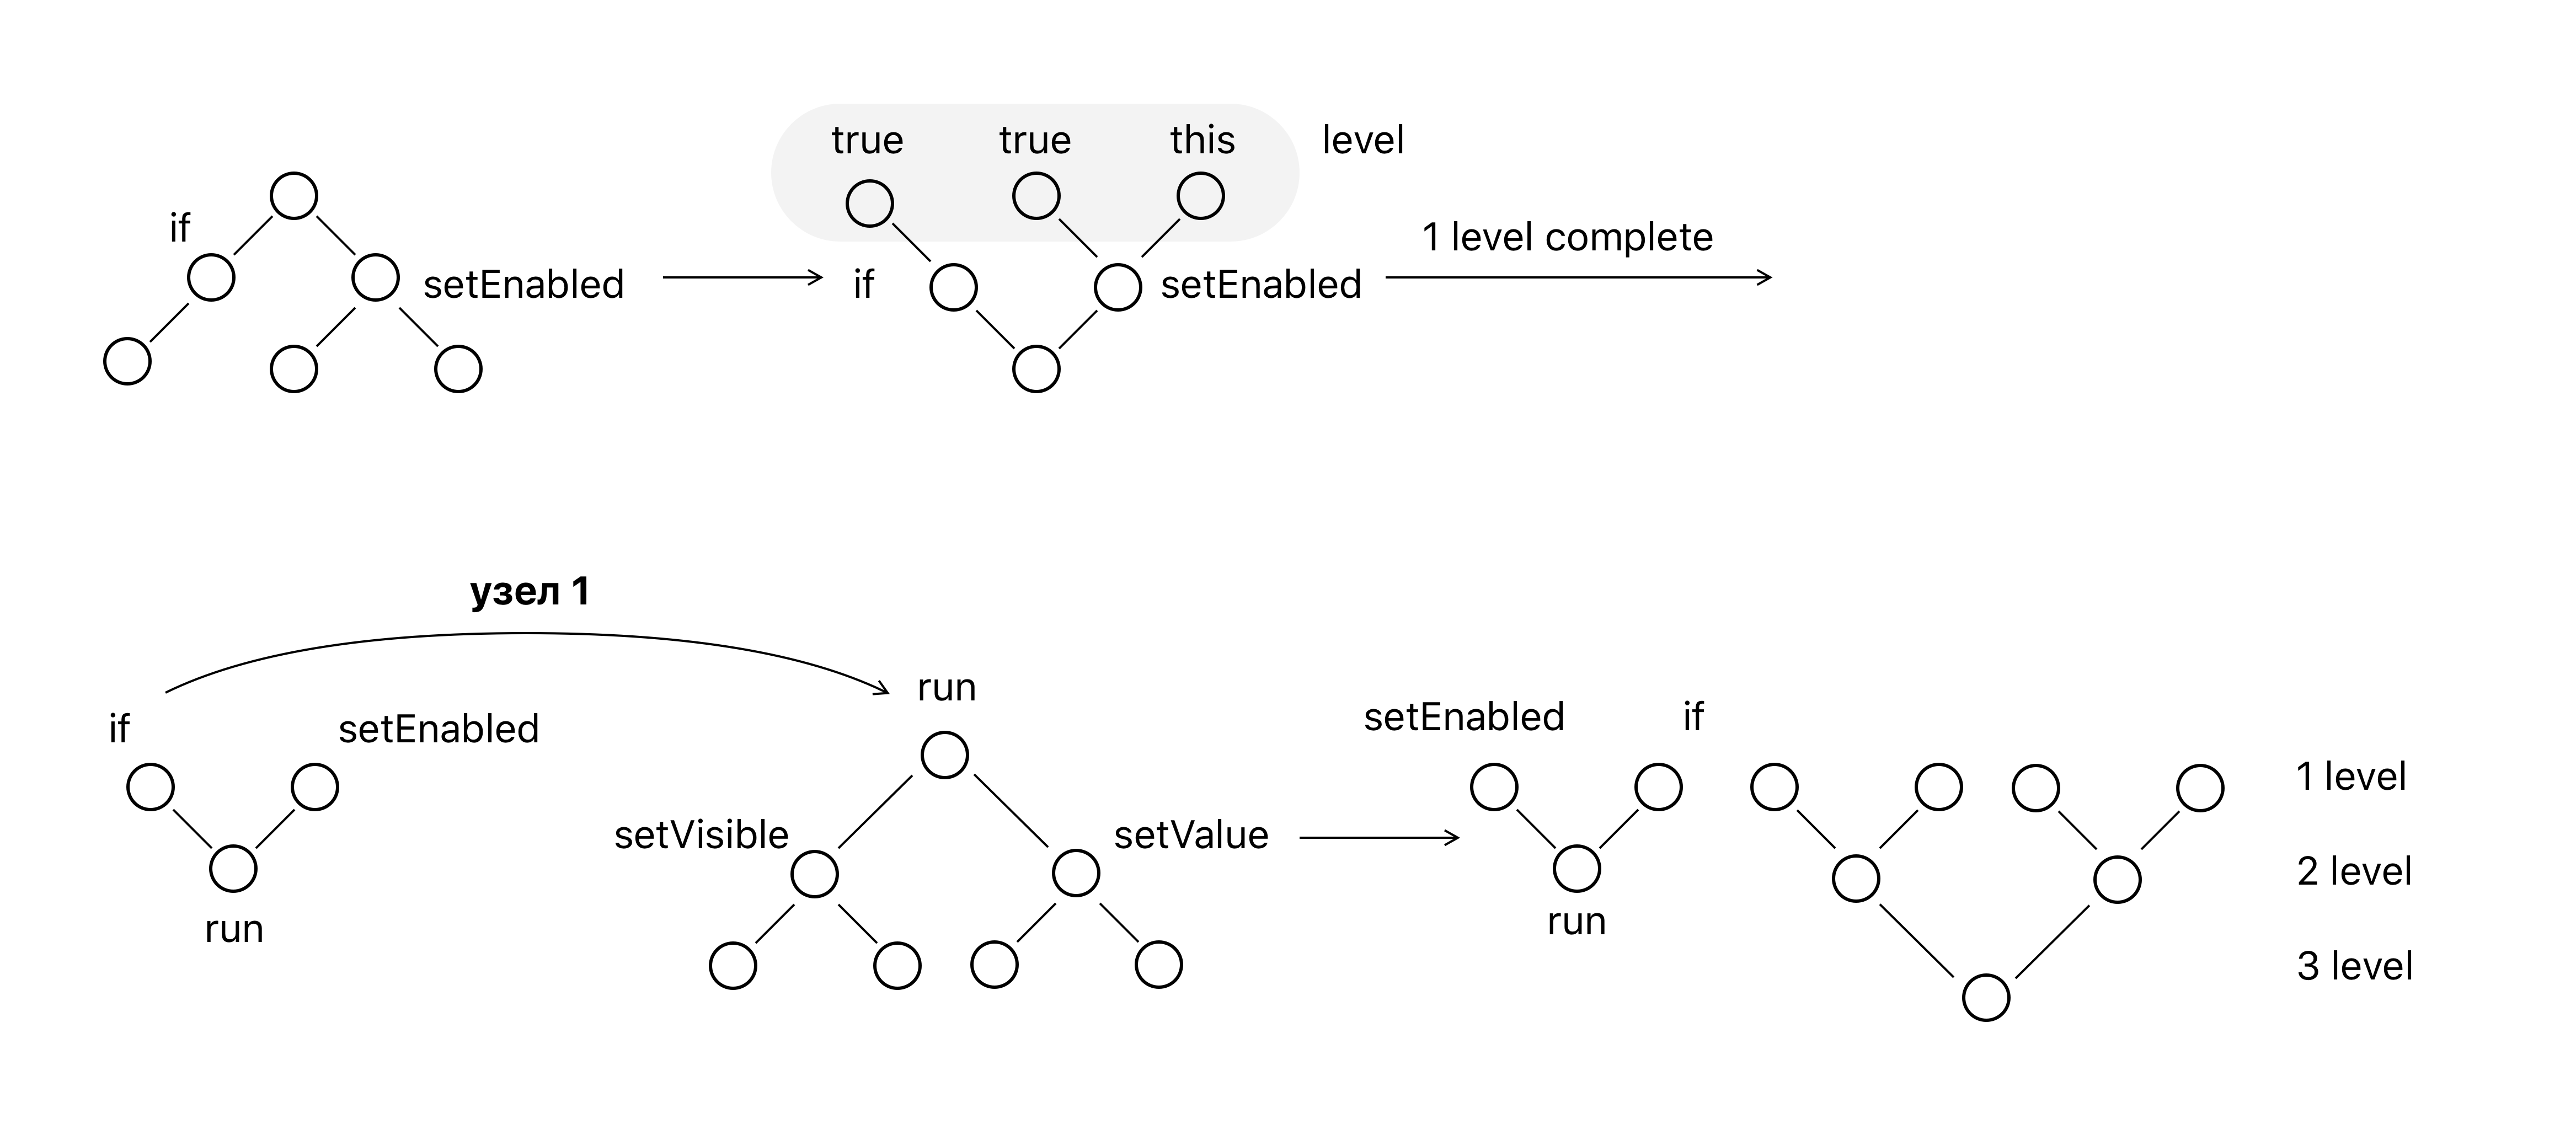
\includegraphics[width=1.0\textwidth]{withIfTree}
	\centering
\end{figure}

Понимая концепции порядка выполнения команд, а также особенности запуска циклов обработки команд можно автоматизировать сколько угодно сложные наборы операций над динамическими формами.

\label{sec:async}
\section{Асинхронные функции}

Помимо функций из стандартной библиотеки которые исполняются синхронно, 
то есть исполнение кода останавливается пока функция не вернет значение, также 
в web интерфейсах, выполняется в процессе браузера, что приводит к блокированию 
пользовательского интерфейса на время выполнения функции.
асинхронные же функции не блокирую поток выполнения браузера, но также блокируют 
выполнение динамического языка. Что примечательно асинхронные функции не блокируют
несколько параллельных команд если они запущены внутри функции $run$.

Асинхронные функции необходимы для вызова автоисполнятора.

Асинхронные функции не имеют специального имени -- они могут быть названы любым именем, которое не входит в список динамических функций стандартной библиотеки(см. \autoref{apx:dlib_doc}).
Функции без нижнего подчеркивания делают запрос к стандартным скриптам, с нижнем подчеркиванием -- 
к скриптам с обработкой формы.

Стандартный вызов функции выглядит так:
\begin{verbatim}
    func([name], [arg0], ... [argN])
\end{verbatim}

$name$ -- имя метода автоисполнятора, arg0...argN аргументы которые передаются в автоисполнятор.

Количество аргументов таких функций не ограничено. Первым аргументом передается название скрипта, 
а последним -- элемент над которым производится выполнение.

Вызов функции с обработкой форму не отличается от обычного вызова функции, но при передаче в автоисполнятор
дополнительным параметром передается вся динамическая форма в формате 3DMap. 
Такие функции всегда возвращают $id$ элемента на которым был вызван, а среда выполнение обрабатывает 
дополнительные параметры которые могут добавить или удалить элемент формы, поменять состояние нескольких элементов
и т.д.  

\subsection{Автоисполнятор}\label{autoexec}

Автоисполнятор или АИ -- представляет собой Task Manager или систему асинхронного выполнения задач. 
Задачи представляют собой скрипты написанные на языке groovy. 
Groovy -- объектно-ориентированный язык программирования разработанный для платформы 
Java как альтернатива языку Java с возможностями Python, Ruby и Smalltalk. 
Каждый скрипт идентифицируется по уникальному имени,
\begin{verbatim}
FRIEND_GET_LIMIT_BY_USER_TPL_DOUBLE. 
\end{verbatim}

Кроме имени скрипт на вход принимает дополнительные параметры. 

\subsection{Обработка ответа от автоисполнятора}

В зависимости от типа вызова функции, автоисполнятор может вернуть структуру $Map$ и $3DMap$.
Структура типа $Map$ представляют собой массив значений <<ключ-значение>>.

\begin{verbatim}
    // JSON 
    [
      { key: "id", value: " }
    ]??????
\end{verbatim}

Такая структура хорошо подходит для обмена данными между элементами формы типа select.

$3DMap$ данная структура данных предназначена для описания изменения в динамической формы.
С ее помощью можно описать добавление, удаление, изменение элементов динамической формы.

Данный формат описывает массив команд который нужно выполнить на динамической формой.
Команды которые поддерживается всеми средами выполнения:

$new$ команда позволяет добавить один или несколько новых элементов.
$attr$ позволяет изменить несколько аттрибутов формы
$value$ устанавливает значение элемента
$valueselected$ устанавливает выбранное значения для элементов типа select
$valuevisible$ устанавливает флаг видимости элемента на дин форме
$valueenabled$ запрещает или разрешает редактирование элемента
$command$ выполняет команду дин языка
$delete$ удаляет элемент с формы
$beforesave$ устанавливает команду которая будет выполнена перед сохранением обращения

Пример ответа сервера в этом формате можно посмотреть в \autoref{apx:3dmap}.

\end{document}